\chapter{Transcription initiation by\textit{Escherichia coli} RNA Polymerase}
\label{chpt:RNAP}


\section{Introduction}
\label{sec:rnap_intro}

The central dogma of molecular biology, formalized by Francis Crick in 1970, describes the flow of genetic information between DNA, RNA, and proteins~\cite{crick_central}. 
Crick's seminal work included the presentation of the first diagram illustrating the central dogma, depicting the possible transfers of information.
Figure 1 from his original paper is presented in Fig.~\ref{fig:central_dogma}A. 
Additionally, Figure 3 of the same publication provided a simplified version of the diagram in which only \enquote{plausible} transfers of information were included based on the scientific understanding at that time. 
This simplified version is shown in Fig.~\ref{fig:central_dogma}B.
In this diagram, Crick deliberately excluded certain arrows, indicating that these particular processes were deemed implausible. 
Furthermore, he used dotted lines to represent \enquote{special transfers} referring to transfers that were considered exceptions or occurred in specific cellular contexts.

\begin{figure}
    \centering
    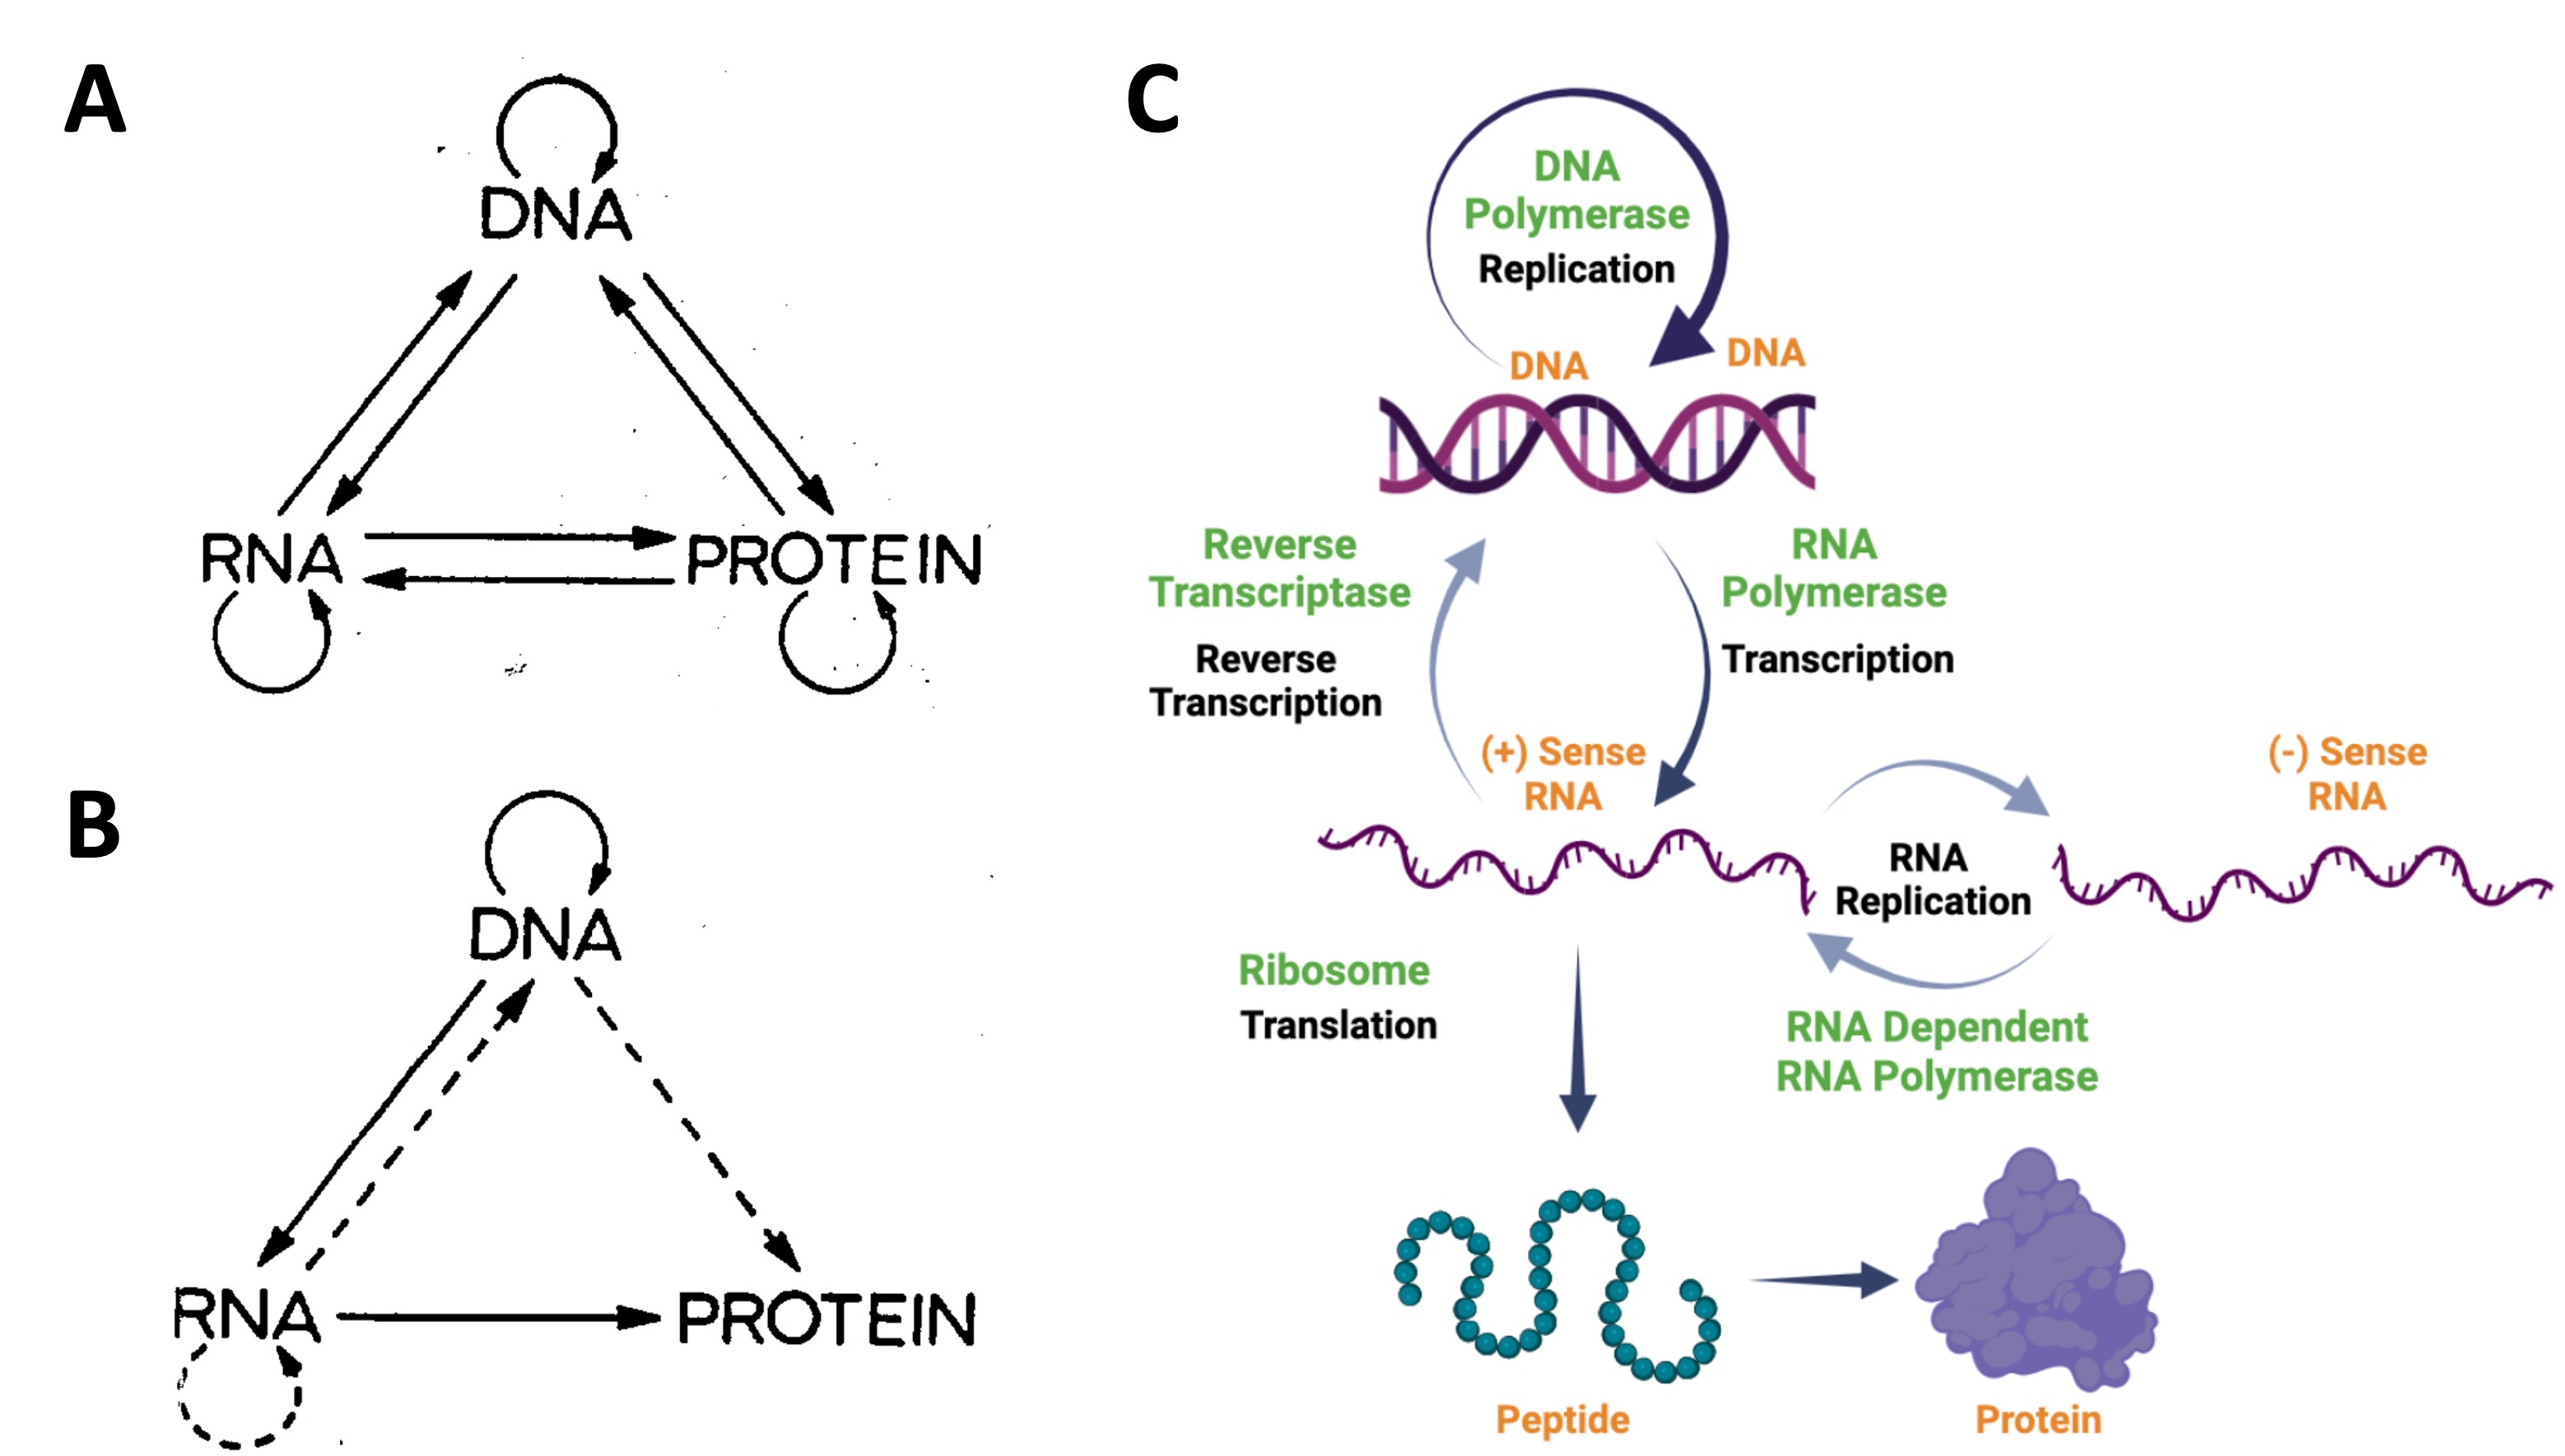
\includegraphics[width=\textwidth]{chapters/figures/central_dogma.jpg}
    \caption{\label{fig:central_dogma}The Central Dogma of molecular biology. 
    A) \enquote{The three families of polymers. They represent the directional flow of detailed sequence information.}~\cite{crick_central}
    B) \enquote{A tentative classification for the present day. Solid arrows show general transfers; dotted arrows show special transfers. ...the absent arrows are the undetected transfers specified by the central dogma.}~\cite{crick_central}
    C) Replication: DNA polymerase is responsible for replication of the DNA genome, where DNA $\rightarrow$ DNA.
    Transcription: RNA polymerase is the enzyme that transcribes the DNA genome into RNA, where DNA $\rightarrow$ RNA. 
    Translation: mRNA produced during transcription is processed and converted into strings of amino acids that fold into proteins, where RNA $\rightarrow$ protein. 
    \enquote{Special transfers} are shown in grey-blue.
    These transfers occur in viral systems.
    Retroviruses utilize an enzyme called reverse transcriptase, that synthesizes DNA from an RNA template, where RNA $\rightarrow$ DNA.
    In some viral systems, replication of the RNA genome and transcription of viral proteins is performed by an enzyme called RNA-dependent RNA polymerase i.e., RNA $\rightarrow$ RNA.
    Figures and captions in A and B were reprinted from Crick's publication \enquote{Central Dogma of Molecular biology}~\cite{crick_central}.
    The author created the cartoon presented in C using BioRender.
    }
\end{figure}

Notably, Crick first presented the idea of the central dogma in 1958. 
However, his 1970 publication formalized the framework, and the significance and foresight of this initial diagram cannot be overstated.
Indeed, the discovery of each of the enzymes involved in these processes resulted in a Nobel Prize.

In 1959 Severo Ochoa and Aurthur Kornberg were awarded the Nobel Prize in Medicine for their discovery of \ac{RNAP} and DNA polymerase respectively. 
Tragically, as has happened many times throughout history, Sylvy Ruth Levy, an accomplished biochemist who worked alongside Kornberg and, not incidentally, was his first wife, later stated that she was \enquote{robbed} after learning that her husband had been awarded the prize~\cite{lenzer_2008}. 
It was Sylvy Ruth Levy who isolated and characterized a contaminating enzyme that inhibited the polymerization reaction~\cite{kornberg_enzymatic_1958}, and therefore also inhibited the discovery of DNA polymerase until she solved the problem.
Without her essential contributions, Kornberg's recognition and subsequent Nobel Prize achievement would not have been possible.

In 2006, almost 50 years later, Aurthur and Sylvy Kornberg's son, Roger Kornberg, was awarded the Nobel Prize for structural determination of eukaryotic RNAP and for elucidating the role of RNAP in the polymerization reaction of RNA. 

Shortly after, in 2009, Venkatraman Ramakrishnan, Thomas A. Steitz, and Ada E. Yonath were awarded the Nobel Prize in Chemistry for their discovery of the structure and function of the ribosome. 
The ribosome is the enzyme responsible for the process of translation, the creation of proteins from \ac{mRNA} i.e., RNA $\rightarrow$ protein, as depicting in
Fig.~\ref{fig:central_dogma}C. 
 
Additionally, the central dogma has been expanded to include reverse transcription, where DNA is synthesized from an RNA template, and RNA replication, where RNA is replicated from an RNA template, shown by the grey arrows in Fig.~\ref{fig:central_dogma}C.
Notably, these \enquote{special} transfers are observed in viral systems, and while these processes occur in the cell, they are not a natural mechanism of \textit{cells} as suggested by Crick.

\section{Transcription initiation by bacterial RNAP}
\label{sec:transcription_initiation}

In bacteria, the transcription of DNA to RNA is performed by RNAP. 
The bacterial system's relative simplicity and conserved nature make it an ideal model for single-molecule studies of RNAP. 
Furthermore, the ability to reconstitute the system \textit{in vitro} provides scientists with precise control over its experimental conditions.
The study of the bacterial RNAP system provides important insights into the broader functions of RNAPs and enhances our understanding of bacterial mechanisms that may become targets for antibacterial medicines.

\subsection{Overview of RNAP structural components}
\label{sec:RNAP_structure}

\begin{figure}
    \centering
    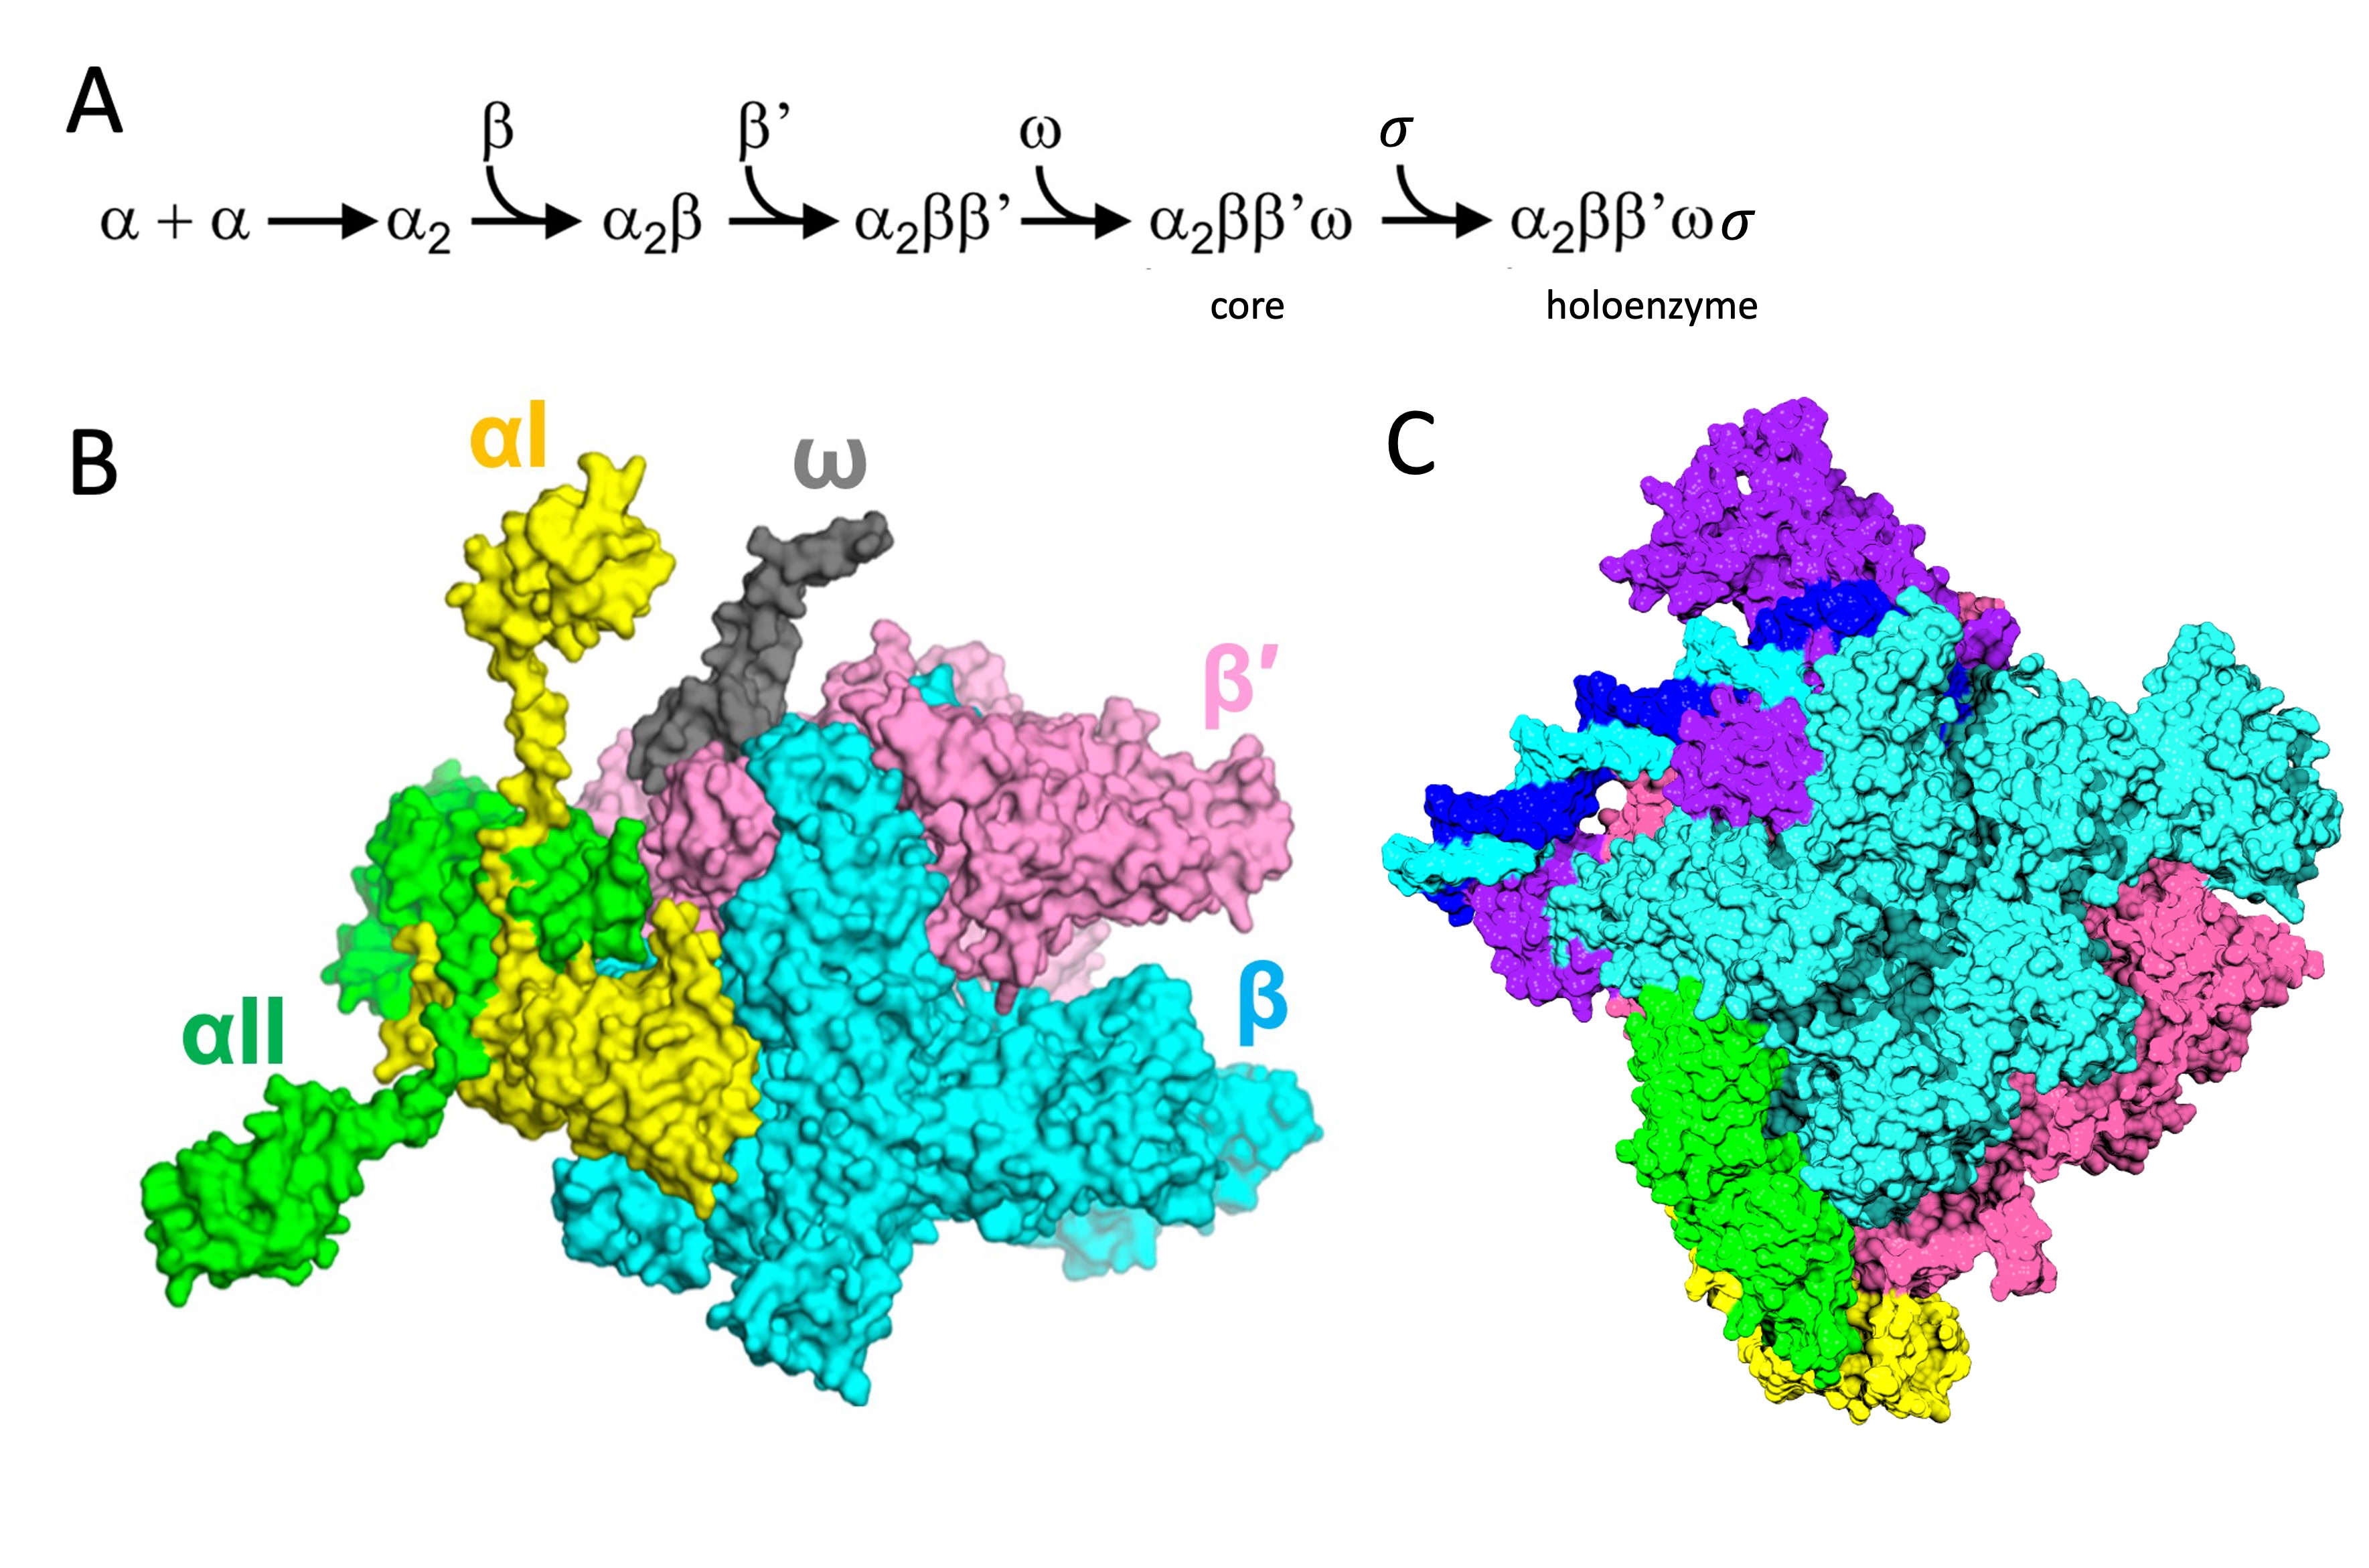
\includegraphics[width=\textwidth]{chapters/figures/RNAP_structure.jpg}
    \caption{\label{fig:RNAP_structure} Structure of RNAP. 
    A) Assembly of the five subunit core enzyme where the $\alpha$ subunits form a dimer which acts as a scaffold for assembly of the three other subunits. 
    The $\beta$ and $\beta'$ subunits associate to the $\alpha$ dimer, followed by $\omega$, forming the catalytically active core enzyme.
    The holoenzyme is formed upon addition of a $\sigma$ factor.
    B) Structure of the assembled RNAP core enzyme ($\alpha_I$: yellow, $\alpha_{II}$: green, $\beta$: cyan, $\beta'$: pink, and $\omega$: gray). 
    \ac{PDB} accession code 4YG2~\cite{murakami_JBC_2013}.
    C) Structure of \textit{\ac{E. coli}} \ac{$RP_o$}, where $\sigma^{70}$ is bound to the RNAP core.
    The holoenzyme is bound to promoter DNA forming an open bubble complex, \ac{$RP_o$} ($\alpha_I$: yellow, $\alpha_{II}$: green, $\beta$: cyan, $\beta'$: pink, and $\omega$: gray, $\sigma^{70}$: purple, \ac{TS}: cyan, \ac{NTS}: blue).
    \ac{PDB} accession code 4YLN~\cite{zuo_steitz_2015}.
    Figures A and B adapted from Ref.~\cite{sutherland_2018}}
\end{figure}

The RNAP core enzyme is composed of five subunits (Fig.~\ref{fig:RNAP_structure}A) and is responsible for the polymerization of RNA using a DNA template and \ac{NTP} substrates.
The RNAP enzyme is often referred to as a crab claw, where the the $\beta$ and $\beta'$ lobes form the DNA-binding site and catalytic center, as can be seen in Fig.~\ref{fig:RNAP_structure}B.
The five-subunit core is conserved across evolution, and spans the archaeal, bacterial, and eukaryotic kingdoms~\cite{murakami_JBC_2013}.
The bacterial system is the simplest, as archeal and eurkaryotic systems are known to have between 11-15 subunits~\cite{werner_2011}. 

RNAP achieves RNA synthesis through the nucleotide addition cycle, wherein each iteration involves the incorporation of an incoming NTP. 
The selection of incoming NTPs is based on their sequence complementarity to the DNA template strand. 
The RNAP active site is composed of two highly conserved \ac{DPBB} domains, one from the $\beta$ subunit and one from the $\beta'$ subunit. 
The DPBB domain of the $\beta'$ subunit contains an aspartic acid triad within the amino acid sequence, -\underline{D}F\underline{D}G\underline{D}-, which plays a critical role in positioning the two catalytic Mg$^{2+}$ ions during the nucleotidyl transfer reaction~\cite{murakami_JBC_2013}.
NTPs enter the active site via the secondary channel, indicated by a small black arrow in Fig~\ref{fig:transcription_cycle}. 
The trigger loop in the $\beta'$ subunit positions the NTPs such that the cannonical Watson-Crick pairing is achieved with the \ac{TS} of the DNA. 
The bridge helix is thought to support the function of the trigger loop during polymerization~\cite{murakami_JBC_2013}.

The \textit{\ac{E. coli}} RNAP core enzyme is transciptionally competent, however promoter sequence specific recognition requires a $\sigma$ factor.
In bacteria, including \textit{\ac{E. coli}}, several $\sigma$ factors exist. 
Among them, the $\sigma^{70}$ factor, or $\sigma^A$ in other bacteria, is a group I factor that plays a crucial role in transcribing primary or \enquote{housekeeping} genes. 
These genes are essential for fundamental cellular functions.
The $\sigma$ factors have highly conserved sequences, suggesting that the function of amino acids in these regions are critical for proper function.

\subsection{The RNAP transcription cycle}
\label{sec:RNAP_cycle}

\begin{figure}
    \centering
    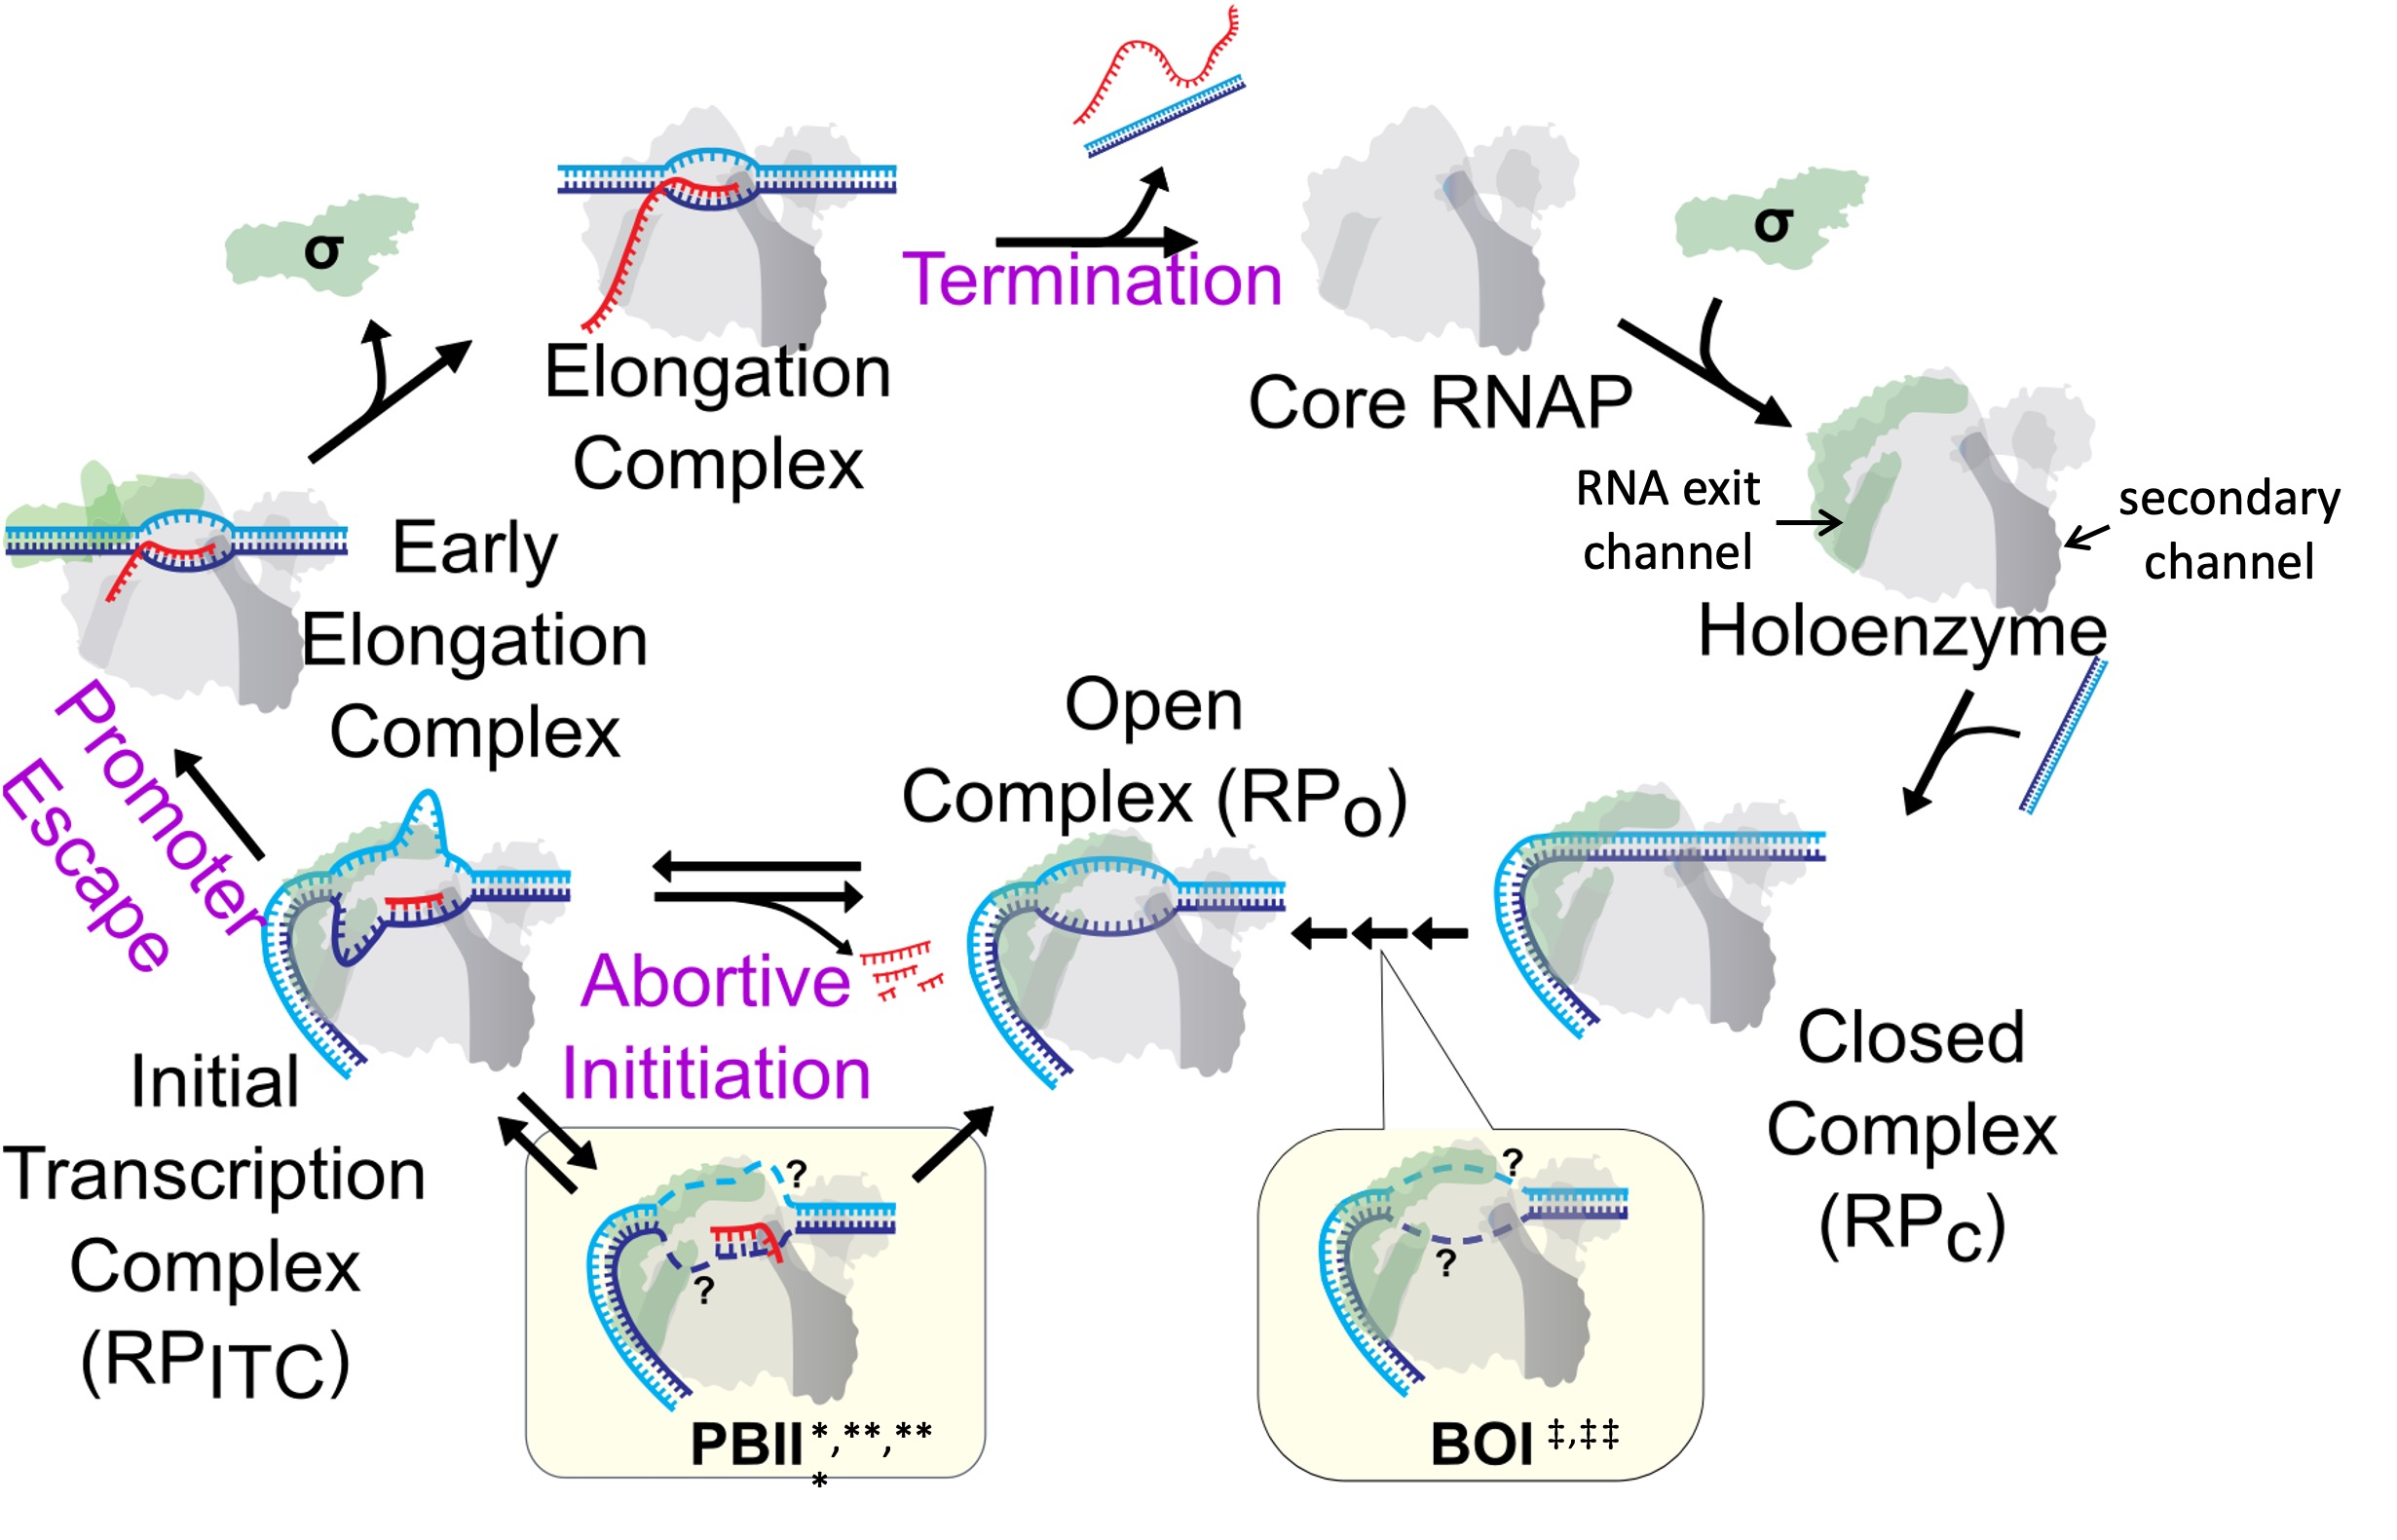
\includegraphics[width=\textwidth]{chapters/figures/transcription_initiation.jpg}
    \caption{\label{fig:transcription_cycle}Bacterial RNAP transcription cycle. 
    The sigma subunit (shown in green) binds to the RNAP core (shown in grey) to form the holoenzyme. 
    The holoenzyme undergoes conformational changes and binds to the promoter DNA, forming the closed complex. 
    The closed complex undergoes isomerization to form the open complex, where the DNA becomes single-stranded. Multiple conformational intermediates \ac{BOIs} (boxed in yellow) can occur during this transition. 
    The open complex proceeds to the initial transcription complex (\ac{$RP_{ITC}$}), during which abortive initiation and paused-backtracked initiation intermediates (\ac{PBIIs}) occur. 
    Late ITC is marked by the displacement of the $\sigma_{3.2}$ loop, allowing the nascent RNA to pass through the RNA exit channel (indicated by a small black arrow).
    The elongation complex is formed, leading to processive elongation and eventually termination. 
    Upon termination, the RNAP core enzyme dissociates from the DNA.
    Figure reproduced from Ref.~\cite{lerner_PNAS_2016}}.
\end{figure}

Transcription by RNAP involves multiple steps. 
Figure~\ref{fig:transcription_cycle} illustrates the transcription cycle of \textit{\ac{E. coli}} RNAP. 
The first step in this process involves a $\sigma$ subunit, shown in green, that binds to the RNAP core, shown in grey, to form the transcriptionally active holoenzyme complex.
Upon binding, the RNAP holoenzyme undergoes conformational changes that allow the $\sigma$ subunit to recognize and tightly bind to a DNA promoter sequence, forming the \ac{$RP_c$}. 

The helicase activity of RNAP unwinds 10-12 \ac{bp} of the double-stranded DNA promoter sequence forming the \ac{$RP_o$} and thus allowing access to the gene region on the \ac{TS} of the DNA. 
Fig.~\ref{fig:RNAP_structure}C shows the crystal structure of the RNAP holoenzyme, where $\sigma^{70}$ is bound to the RNAP core enzyme. 
Multiple \ac{BOIs}, boxed in yellow in Fig.~\ref{fig:transcription_cycle}, are thought to occur during this transition. 
These \ac{BOIs} are fast, inter-converting conformations along the \ac{$RP_c$} $\rightarrow$ \ac{$RP_o$} path that occur on the order of 0.5 - 5.0 ms~\cite{lerner_JCP_2018, robb_JMB_2013}.

Upon formation of \ac{$RP_o$} RNA polymerization begins, and the \ac{$RP_{ITC}$} is formed.
During this important transition, a process called abortive initiation occurs where multiple failed attempts of transcription occur before the holoenzyme escapes the high affinity promoter region, whereby the enzyme can move processively into elongation. 
Due to the compaction stress of DNA scrunching into the transcription bubble~\cite{kapanidis_science_2006} and subsequent backtracking and nucleotide excision, the process of abortive initiation results in short transcripts $\sim2-7$ nucleotides long, where the abortive transcripts are shown in red in Fig.~\ref{fig:transcription_cycle}.
The conformational intermediates that occur along the \ac{$RP_o$}  $\rightarrow$ \ac{$RP_{ITC}$} transition are known as \ac{PBIIs}, boxed in yellow in Fig.~\ref{fig:transcription_cycle}. 
These \ac{PBIIs} are known to occur on the order of $\sim20$s~\cite{kapanidis_science_2006,lerner_PNAS_2016,lerner_transcription_2017}.
Pausing during transcription postpones the transition to elongation.
The process of abortive initiation and pausing appears to be highly inefficient, leading to the speculation that it may serve as a fidelity mechanism. 
This hypothesis gains even more strength when we consider that RNAP lacks a dedicated exonuclease domain.

Late \ac{$RP_{ITC}$} is characterized by the displacement of the $\sigma_{3.2}$ loop from the RNA exit channel, allowing the nascent RNA exit the complex, as shown in the Fig.~\ref{fig:transcription_cycle} diagram.
This processes, where the RNAP holoenzyme breaks contact with the tightly bound promoter region, is referred to as promoter escape. 
The Fig.~\ref{fig:transcription_cycle} diagram shows a structural change where a region of the $\sigma^{70}$ factor is displaced from the RNA exit channel and moves above the open bubble region.
Following the escape of the promoter region of the DNA, the holoenzyme proceeds to processive elongation, where the transition of early elongation to elongation is typically marked by the dissociation of the $\sigma$ factor. 
However, in past studies we have observed that the $\sigma^{70}$ factor does not always dissociate~\cite{kapanidis_MolCell_2005}.

Following elongation, the reaction terminates.
Termination is characterized by the re-formation of the closed bubble at the original $RP_o$ complex location, allowing for the cycle to begin again, as shown in the Fig.~\ref{fig:transcription_cycle} diagram.

\subsection{\label{sec:promoter_escape} 
Unraveling the role of the $\sigma_{3.2}$ loop during promoter escape}

\begin{figure}
    \centering
    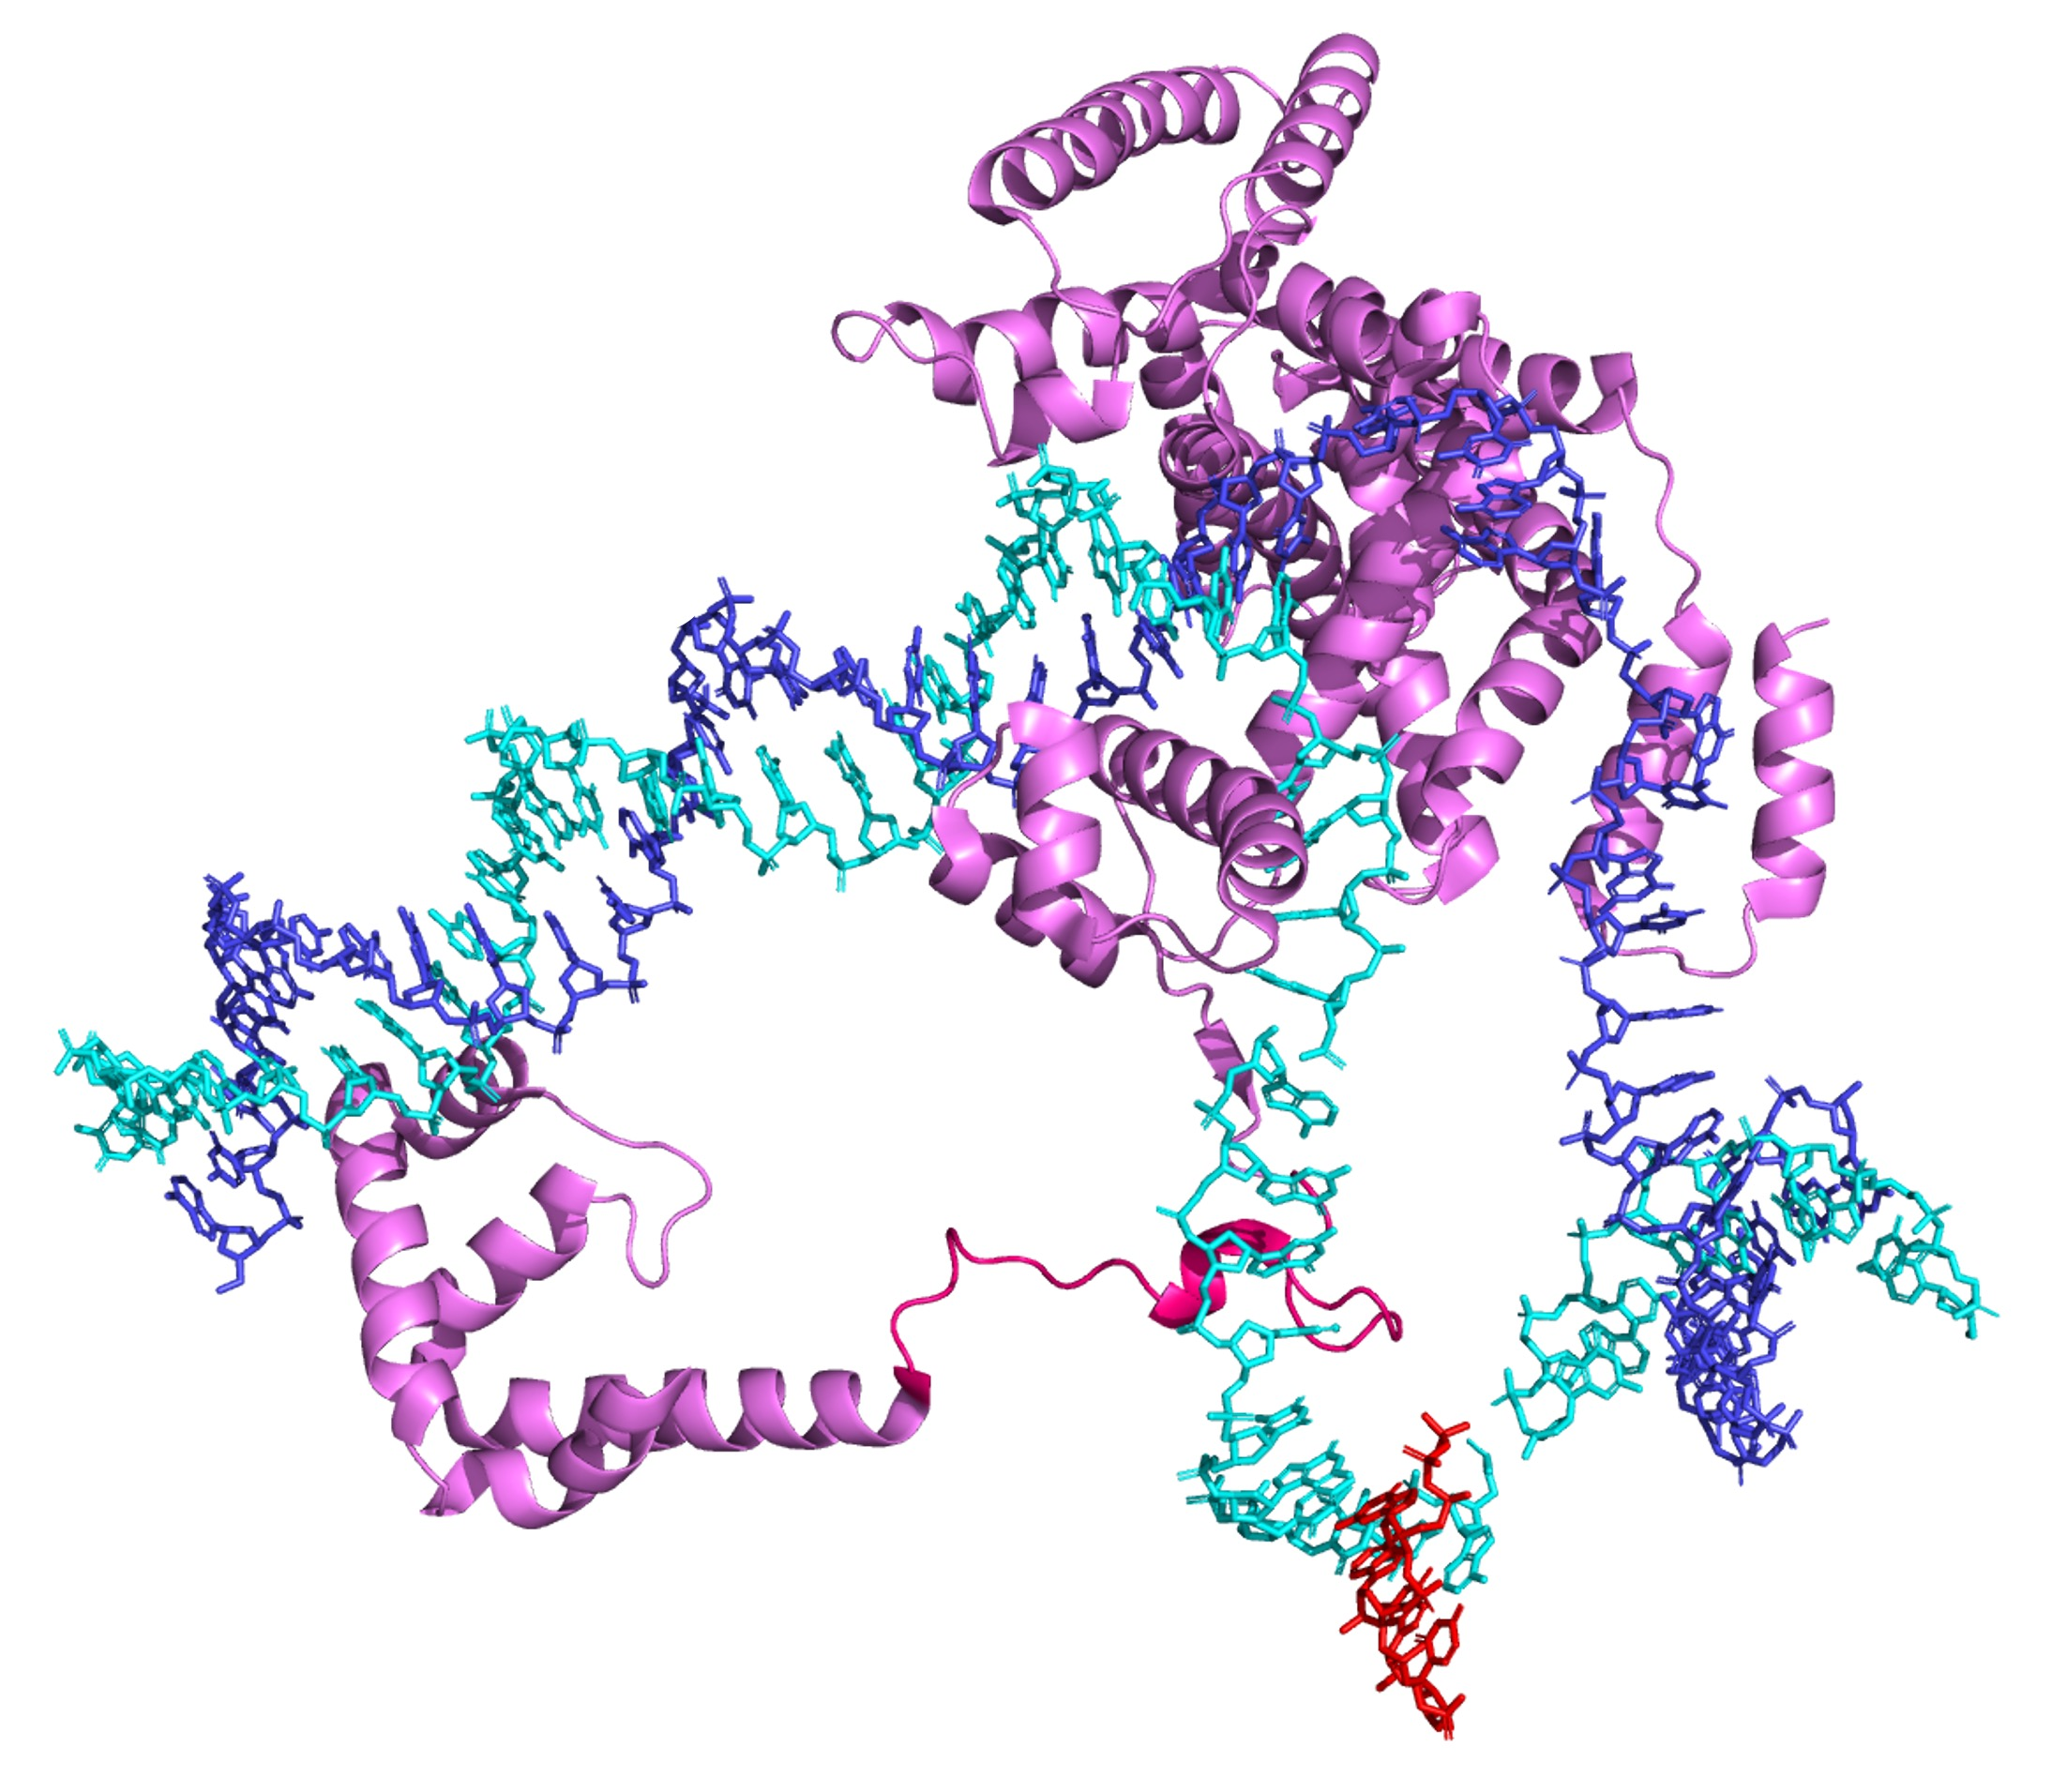
\includegraphics[width=\textwidth]{chapters/figures/sigma_structure.jpg}
    \caption{\label{fig:sigma_structure} 
    Structure of the $\sigma^{70}$ in the open-bubble complex.
    Structure of the $\sigma^{70}$ factor, shown in purple, in complex with the open promoter DNA, where the \ac{NTS} is shown in blue and the \ac{TS} is shown in cyan.
    A nascent tretranucleotide in the catalytic center is shown in red.
    The $\sigma_{3.2}$ loop is highlighted in magenta.
    Notably, I have removed the RNAP core enzyme from the x-ray crystal structure to highlight the conformation of $\sigma^{70}$ and the $\sigma_{3.2}$ loop in complex with the DNA.
    \ac{PDB} accession number 4YLN~\cite{zuo_steitz_2015}.
    }
\end{figure}

The $\sigma^{70}$ factor is essential for recognition of promoter sequences during initiation and is thought to be involved in abortive initiation and promoter escape. 

$\sigma^{70}$ binds to the DNA and bends it into the active site, forming a single-stranded open-bubble region.
The $\sigma_{3.2}$ region, indicated in magenta in Fig.~\ref{fig:sigma_structure}, is a flexible loop that extends into the RNA exit channel. 
Its amino acid sequence is conserved across evolution and contains positively charged residues.

It is hypothesized that the positive electrostatic interaction between the aspartic acid residue in the $\sigma_{3.2}$ loop and the nascent RNA guides the RNA into the RNA exit channel~\cite{zuo_steitz_2015}. 
As the nascent RNA lengthens, tension accumulates at the interface between the loop and the RNA, ultimately leading to the loop obstructing the RNA exit channel, as shown in the crystal structure in Fig.~\ref{fig:sigma_blockage}.

Based on this evidence, it is hypothesized that the mechanism of transition to promoter escape involves the displacement of the $\sigma_{3.2}$ loop, allowing the nascent RNA to exit.

Once the $\sigma_{3.2}$ loop is removed from the RNA exit channel, the transition to elongation proceeds, and the enzyme polymerizes RNA processively, as depicted in Fig.~\ref{fig:transcription_cycle}. 
However, the removal of the $\sigma_{3.2}$ blockage has not yet been observed. 

\begin{figure}
    \centering
    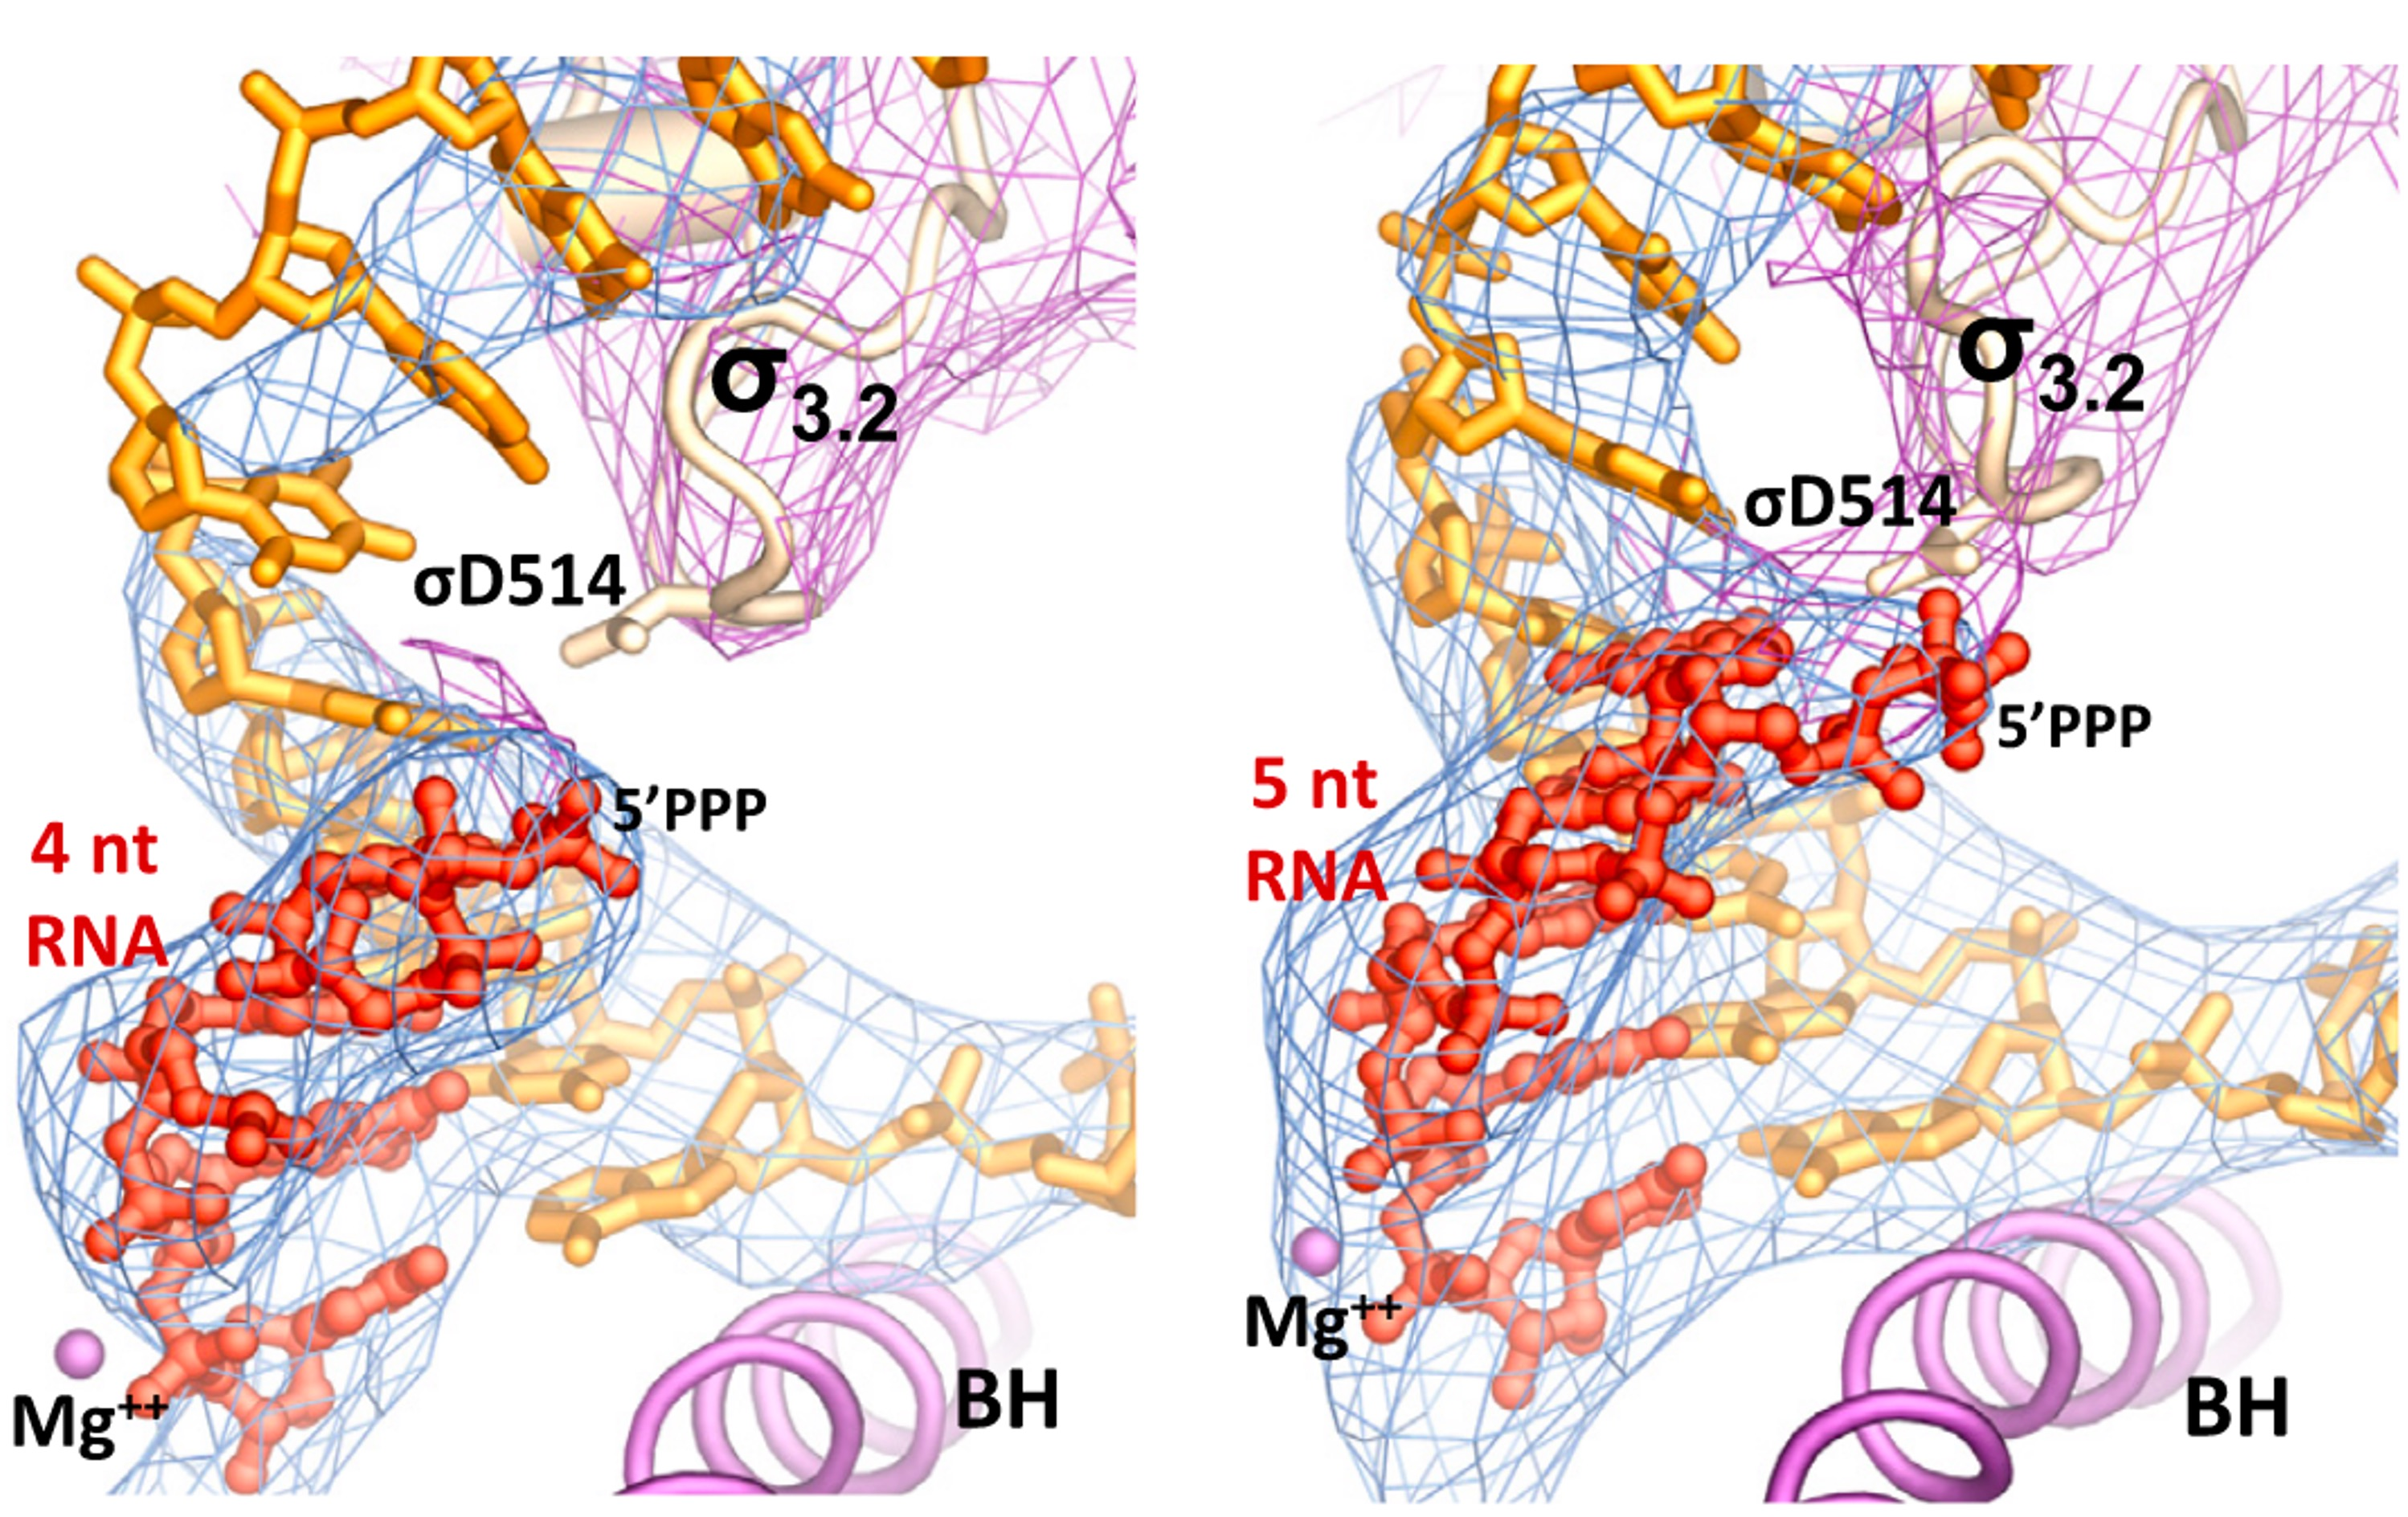
\includegraphics[width=\textwidth]{chapters/figures/sigma_blockage.jpg}
    \caption{\label{fig:sigma_blockage} 
    Blockage of the RNA exit channel by the $\sigma_{3.2}$ loop.
    Left: $\sigma_{3.2}$ loop in complex with an RNA tetranucleotide.
    Right: RNA pentanucleotide interacts with the positively charged residue D514, resulting in a build up of tension at the interface between the nascent RNA and the $\sigma_{3.2}$ loop.
    The bridge helix and the Mg$^{2+}$ ion of the active site are shown for included for structural context.
    The blue meshes in the figure represent the electron density map calculated without the nucleic acids, while the purple meshes represent the electron density map of the $\sigma_{70}$ factor.
    Figure reproduced from Ref.~\cite{zuo_steitz_2015}.
    }
\end{figure}

\section{\label{sec:research_focus} Research focus}

Transcription serves as a crucial checkpoint in gene regulation and ultimately determines a cell's phenotype. 
Throughout this work, I focus on the non-equilibrium dynamics of RNAP during transcription initiation and promoter escape. 
By studying Bacterial RNAP, a simplistic yet informative system conserved throughout evolution, I am poised to provide valuable insights about this essential process. 
Specifically, bacterial RNAP studies can inform the development of antibiotics and expand the phase space for drug discovery. 

Current structural determination methods lack the capability to observe short-lived, freely-diffusing conformational intermediates. 
Gold standard techniques such as cryo-EM or x-ray crystallography require that the molecules be either surface bound, frozen, crystallized, or both. 
These methods achieve angstrom length-scale resolution, however they come at the cost of immobilizing an otherwise freely moving molecule. 

To address the challenge of conducting structural studies under freely-diffusing conditions, where molecules have unrestricted movement and may sample various microstates, I have developed a high-throughput method that enables single-molecule studies using fluorescence spectroscopy.
By expanding the capabilities of the typical single-molecule FRET microscope, I have developed a high-throughput single-molecule FRET platform to investigate the dynamics of RNAP during non-equilibrium studies of transcription initiation.
Using this platform, I aim to capture the structural transitions of RNAP as it undergoes various conformational states, such as the formation of the closed complex, the isomerization to the open complex, and the transition to elongation. 
These transitions involve the formation of short-lived conformational intermediates, such as \ac{BOIs}, \ac{PBIIs}, and perhaps others, which have not yet been observed or structurally characterized.

By studying the dynamics of RNAP during promoter escape, I aim to understand the mechanisms underlying the displacement of the $\sigma_{3.2}$ loop, which allows the nascent RNA to exit the RNA exit channel. 
This process is thought to play a crucial role in abortive initiation, and understanding it will shed light on the mechanism of transcription and provide insights into the regulation of gene expression.

By developing a high-throughput single-molecule fluorescence spectroscopy platform, I aim to observe and capture the structural transitions of RNAP in real-time. 
This approach provides a valuable advancement in structural determination, as it allows for the observation of fast-moving intermediates. 
By solving the structure of RNAP as it progresses along its kinetic trajectory, I hope to gain a deeper understanding of the transcription process and contribute to the development of novel therapeutic strategies.

%%%%%%%%%%%%%%%%%%%%%%%%%%%%%%%%%%%%%%%%%%%%%%%%%%%%%%%%%%

%\begin{table}[ht]
%    \begin{tabular}{l|l}
%        \textbf{left column} & \textbf{right column} \\ \hline
%        entry1 & entry2 \\
%        entry3 & entry4
%    \end{tabular}
%    \caption{An example table with things in it. Take a look at https://www.latex-tables.com/ for a relatively-easy latex table generator. Other options include https://truben.no/table/old/ and https://www.tablesgenerator.com/, but you'll find others online, too!}
%    \label{tab:my-table}
%\end{table}



